\documentclass[tikz,border=8pt]{standalone}
\usepackage[T1]{fontenc}\usepackage{lmodern}
\usetikzlibrary{arrows.meta,positioning}
\begin{document}
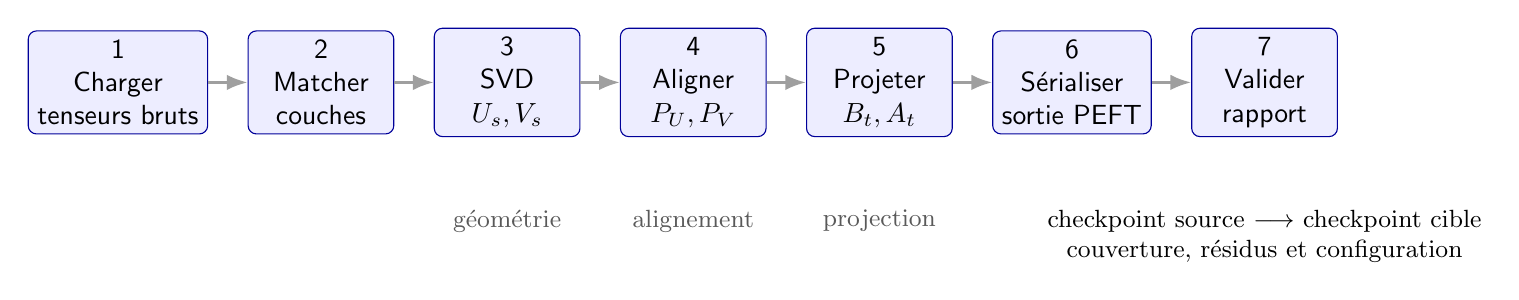
\begin{tikzpicture}[font=\sffamily,>=Latex, node distance=5mm,
 stepbox/.style={draw=blue!60!black,fill=blue!7,rounded corners=3pt,minimum width=1.85cm,minimum height=1.0cm,align=center}, arr/.style={-{Latex},draw=gray!75,line width=1pt}]
\node[stepbox] (io) {1\\Charger\\tenseurs bruts};
\node[stepbox,right=of io] (match) {2\\Matcher\\couches};
\node[stepbox,right=of match] (svd) {3\\SVD\\$U_s,V_s$};
\node[stepbox,right=of svd] (align) {4\\Aligner\\$P_U,P_V$};
\node[stepbox,right=of align] (project) {5\\Projeter\\$B_t,A_t$};
\node[stepbox,right=of project] (save) {6\\Sérialiser\\sortie PEFT};
\node[stepbox,right=of save] (valid) {7\\Valider\\rapport};
\foreach \a/\b in {io/match,match/svd,svd/align,align/project,project/save,save/valid} \draw[arr](\a)--(\b);
\node[below=8mm of svd,font=\small,text=gray!70!black] {géométrie};
\node[below=8mm of align,font=\small,text=gray!70!black] {alignement};
\node[below=8mm of project,font=\small,text=gray!70!black] {projection};
\node[below=8mm of valid,font=\small,align=center] {checkpoint source $\longrightarrow$ checkpoint cible\\couverture, résidus et configuration};
\end{tikzpicture}
\end{document}
